\Chapter{A játék bemutatása}

\Section{OpenTTD bemutatása}

Az OpenTTD egy nyílt forráskódú szimulációs játék amit a kilencvenes években a MircoProse által fejlesztett Transport Tycoon Deluxe alapján hoztak létre \cite{openttd}. A játék célja egy olyan fuvarozó cég felépítése ami a lehető legmagasabb profitot tudja generálni minél több rakomány lehető legoptimálisabb elszállításának köszönhetően. A játékban több fajta járművel is lehetőség van a rakományok elszállítására: közúti járművek (buszok, furgonok), légi járművek (repülők, helikopterek), vasúti járművek (vonatok, vagonok) és vízi járművek (hajók). Az rakományok amelynek a szállítására lehetőség van az alapértelmezett játék beállítások mellett a következők: utasok, levelek, szén, vasérc, acél, fa, olaj, állatok, gabona és áruk. Ezek közül a az utasokat és a leveleket városok között tudjuk szállítani, az árukat pedig a városokba tudjuk elszállítani különböző feldolgozó gyárakból. A többi rakománynak saját forrása és célja van, amelyek bányák vagy gyárak formájában jelennek meg. Mivel a játék teljesen nyílt forráskódú, így a játék bármilyen működése befolyásolható, vagy bővíthető. Erre a játékon belül találunk is opciót, ahol más felhasználók által készített szkripteket adhatunk hozzá a játékhoz. Az egyszerűség kedvéért a továbbiakban csak az alapjáték szabályairól lesz szó.

A játékban a versengés online módban más játékosok, offline módban pedig gépi ellenfelek konkurens cégeiben jelenik meg. Akár egyedül akár ellenfelek ellen játszunk, a játékvilág szabályai ugyanazok. A játék legfontosabb eleme a gazdaság szimulálása, ami egy új játék kezdetekor, már a legelejétől főszerepet kap, egy banki kölcsön formájában. Ez a kölcsön adja meg a játékos kezdő tőkéjét, aminek a helyes befektetésével kell profitot generálnia, hogy később a kölcsönt visszafizesse. Ha a játékos nem képes tartani a lépést a kölcsön részleteivel, vagy esetleg túlköltekezik, abban az esetben a cége csődbe megy és véget ér számára a játék. A megfelelő infrastruktúra kiépítése nem feltétlen olyan egyszerű mint gondolnánk. A megépített utak és sínek, megállók és garázsok után karbantartási költséget, valamint a járművek után pedig fenntartási költséget kell fizetnie a játékosnak, amik mind megnehezítik a pénzügyi helyzetét. Emellett, a városok önkormányzatai befolyással rendelkeznek afelől, hogyha a területükön belül szeretnénk építkezni vagy rombolni, és konkurens cégek akár szerződhetnek egyes önkormányzatokkal, kizárólagos építési engedélyért. A városokon kívül pedig a bányák, gyárak is folyamatosan változnak, attól függően, hogy mennyire aktívan vannak kihasználva, vagy véletlenszerű események hatására. Például, ha három szénbánya közel helyezkedik el egymáshoz képest, de a játékos csak kettőből szállítja el a kitermelt mennyiséget, idő elteltével a harmadik bánya termelése csökkenhet, később akár csődbe is mehet és bezárhat. Ennek a hatására, a másik két bánya termelése pedig növekedhet. Több véletlenszerű esemény is befolyásolhatja még a játékmenetet, egyes önkormányzatok támogatást adhatnak ki bizonyos útvonalak kiépítésére, vagy a játékbeli idő előrehaladtával, egyre nő a légi utazás elfogadottsága, bizonyos rakományok szállítási értéke véletlenszerűen növekedhet vagy csökkenhet. Az idő haladtával új járművek jelennek meg, amelyek modernebbek, effektívebbek, nagyobb a kapacitásuk, és ugyanakkor a régi járművek idősödnek, lerobbanhatnak és balesetben is lehet részük. Ezért ahhoz hogy a legtöbbet hozza ki a járművekből, a játékosnak ezeknek az időszakonkénti karbantartására is figyelmet kell szánnia.

A játék körülményeit a pálya generálásával tudjuk befolyásolni különböző módokon. Beállítható a pálya mérete, ami 64x64-től egészen 4096x4096-ig állítható. Ez természetesen  jelentősen megváltoztatja a városok és iparok számát a térképen, amelyek sűrűségét egyébként van lehetőség külön is beállítani. Emellett állítható a pálya domborzata is, egészen lapostól, ahol általában az egész pályán csak 1-2 magassági eltérés lesz, a nagyon dombos-ig, ahol nagy szintkülönbségek lehetnek, amik természetesen megnehezíthetik az útvonalak tervezését, vagy költségét. Egyéb “földrajzi” opció ami elérhető, az a folyók/tavak sűrűsége és a tengerszint magasságának beállítása, valamint megszabhatjuk, hogy a pálya szélein tengert vagy szárazföldet szeretnénk. Valamint az utolsó lényeges beállítás a kezdés éve, ami hatással lesz a játékos számára elérhető járművekre, valamint technológiákra.

A videojátékok többségében nagy jelentősége van a mesterséges intelligenciának, mint például egy a számítógép által irányított karakter, vagy egy ellenfél. Az OpenTTD esetében a mesterséges intelligencia a számtalan befolyásolható tulajdonság és azok komplexitása miatt szinte végtelen lehetséges megvalósítási lehetőséget tár a fejlesztő elé. 

\Section{A játék célja}

A játékos több fontos döntés előtt áll, már a játék kezdetétől fogva. El kell döntenie milyen módon szeretne játszani, milyen járművekkel szeretné megvalósítani a rakományok szállítását, milyen rakományt szeretne szállítani, a hálózatot hogyan szeretné kiépíteni, milyen úton fogja fedezni a kölcsön törlesztési díját, hosszú távon milyen új módszereket szeretne megvalósítani.

A játékmód alatt értem azt, hogy esetleg csak közúti járművekkel szeretne foglalkozni, vagy csak vasútival stb., vagy csak városok között szeretne szállítani, így csak utasokat és leveleket tud, vagy pedig csak gyárak között, vagy akár mindenből szeretné kivenni a részét.

A hálózat kiépítése alatt arra gondolok, hogy például, az út- vagy vasúthálózatot olyan módon építjük meg, ami a valósághoz hasonlít, vagy mindenhol csak a leggyorsabb útvonalakat építjük meg. Szeretnénk e összekötni minden várost vagy gyárat és kihasználni azokat, vagy csak néhányra fókuszálunk. Valamint egy vasúthálózatot nem ugyan olyan módon építünk meg mint egy úthálózatot, érdemes odafigyelni a különböző járművek sajátosságaira. Erre néhány példa, az út kétsávos és kétirányú, de a vasút egy vágányos de lehet kétirányú. A vonatok meg tudnak fordulni egy helyben állomásokon, a közúti járművek viszont nem, azoknak fordulók kiépítésére van szükség. Egyéb fontos döntés hálózatok építésénél, ha például kevesebb városra fókuszálunk utasok és levelek elszállításával, azok a városok, gyorsabban fognak növekedni, mintha minden városban egyesével építenénk ki az útvonalakat. A nagyobb méretű városok pedig több utashoz és levélhez vezetnek, amiből később több profitot tudunk szerezni.

A kölcsön fedezésére is több módszer lehetséges. A játék kezdetén érdemes lehet korlátozni a terjeszkedést pár kisebb, profitáló útvonalra, amíg a kezdeti kölcsönt visszafizetjük, és aztán vállalni kockázatosabb fejlesztéseket. De stratégia lehet az is, hogy a kezdeti kölcsön mellé, felvesszük a maximális kölcsön mennyiséget amit a játék megenged, és sokkal nagyobb, tágabb infrastruktúra kiépítésére kezdünk, ami rövid távon nem annyira hatékony mint a lassú terjeszkedés, de hosszú távon sokkal nyereségesebb lehet.

Végső soron pedig, mivel a játék környezete interaktív, kérdés lehet a játékos számára hogy hogyan tud a változásokhoz alkalmazkodni. Például jó módszer lehet az önkormányzati támogatások “levadászása” mivel lehetséges, hogy egy egyébként nem túl nyereséges útvonalra a támogatással már sokkal inkább megéri figyelmet fordítani. De ez ellen mehet a korábbiakban megemlített játékterveknek, kiindulva a “csak utasok és levelek” példából, ha a támogatás mondjuk szén szállítására szól, akkor lehet egyébként nyereséges lenne a játékos számára, de nem része a játéktervének. Ugyan így érdemes figyelmet fordítani más játékosokra is legyen az számítógép, vagy valósa a játékos játékos. Ha azt látja hogy az ellenfele csak a városokkal foglalkozik, abban az esetben érdemes lehet neki a bányákra, gyárakra koncentrálni, mivel ott kevesebb a versengés, így több rakomány áll rendelkezésre amiket elszállíthat.

\Section{A játékfelület bemutatása}

A játékot elindítva a főmenü (\ref{fig:menu}. ábra) fogadja a felhasználót. Innen elérhet minden funkciót amire a játék kezdete előtt szüksége lenne. Az "Alapbeállítások" menüpontban beállítható a játék felülete, és játékot befolyásoló tényezőket is. A felület betűméretét, nyelvét, az ablak nagyságát tudjuk beállítani. A játék tényezőire vonatkozó beállítások, a bal vagy jobb kormányos járművek használata, a játék pénzneme és a városok neveinek nyelve.

\begin{figure}[h!]
	\centering
	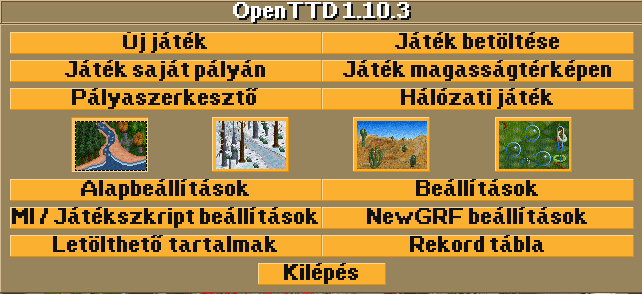
\includegraphics[scale=0.8]{images/menu.png}
	\caption{A játék főmenüje}
	\label{fig:menu}
\end{figure}

A "Beállítások" menüpontban már a játék szabályaira tudunk kihatni. Például tudunk infláció szimulálást be vagy ki kapcsolni, a térképgenerálás paramétereit tudjuk változtatni, a katasztrófákat tudjuk ki- és bekapcsolni, állítani az előfordulásuk gyakoriságát stb.

Az "MI/Játékszkript beállítások" menüpontban (\ref{fig:mibeall}. ábra) tudjuk beállítani, hogy egyjátékos módban, hány AI-t szeretnénk a játékunkban, valamint milyen gyakorisággal jelenjenek meg, és ha erre a fejlesztő lehetőséget ad, az AI kalibrálására is van lehetőség, hasonlóan, az egyéb játékszkripteket is itt tudjuk hozzáadni a játékunkhoz és tudjuk őket beállítani. A bal felső sarokban lévő számláló állításával van lehetőségünk növelni az ellenfelek számát, alapértelmezetten a játékban előforduló AI véletlenszerű lesz, de a hely kiválasztásánál be tudjuk állítani egy konkrét AI-t is.

\begin{figure}[h!]
	\centering
	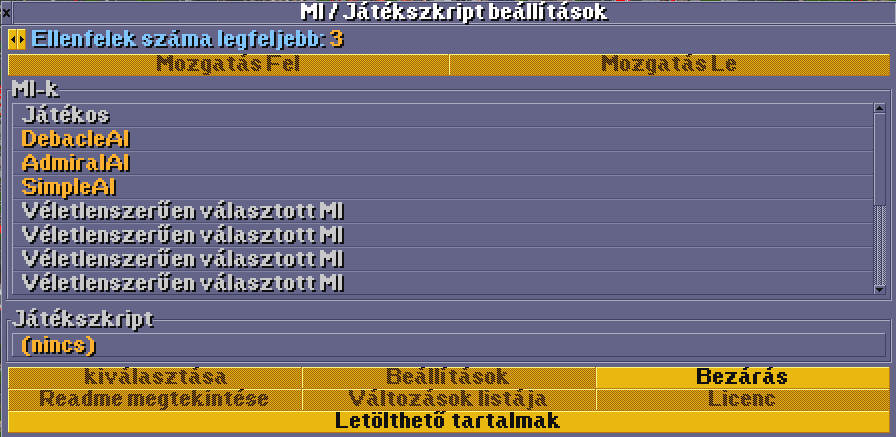
\includegraphics[scale=0.6]{images/mibeall.png}
	\caption{Az MI/Játékszkript beállítások ablak.}
	\label{fig:mibeall}
\end{figure}

A "Letölthető tartalmak" menüpontban van lehetőségünk kibővíteni az alapjátékot különböző szkriptekkel, AI-okkal, hang és grafikai csomagokkal és egyéni térképekkel. Mindezt a BaNaNas repository segítségével tudjuk megtenni a játékon belül, erről későbbiekben lesz még szó \cite{openttdbananas}. 

A menü többi pontja magától értetődő, vagy nem fontos a játékmenet szempontjából. Egy új játék megkezdéséhez egy pályát kell generálnunk, vagy egy korábbit betöltenünk a megfelelő menüpont kiválasztásával. A menü közepén látható négy kép, a különböző játék éghajlatra vonatkozik. Balról az első az alapvető beállítás, a mérsékelt. A dolgozat ennek a körülményeiben fog továbbhaladni. Az "Új Játék" menüpont kiválasztása után, a képek közül kiválasztott játékszabályokkal történő pályagenerálás menüjébe(\ref{fig:generalas}. ábra) kerülünk, ahol a képek újra megjelennek és lehetőségünk van ismét változtatni. Itt tudjuk beállítani, hogy a pálya mennyire legyen dombos, milyen gyakorisággal forduljanak elő városok, gyárak, folyók és hogy a játék milyen dátumon induljon el.

\begin{figure}
	\centering
	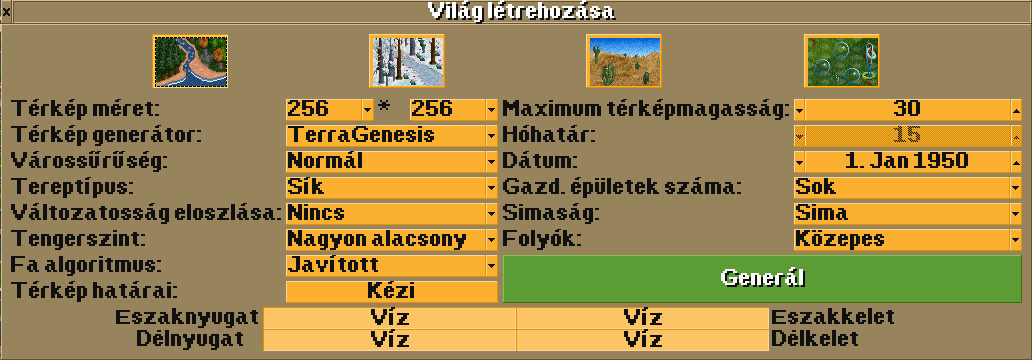
\includegraphics[scale=0.5]{images/generalas.png}
	\caption{Új játék kezdeténél a pályagenerálás beállításai.}
	\label{fig:generalas}
\end{figure}

A zöld "Generál" gomb lenyomása után, egy véletlenszerű seed szerint generál nekünk egy pályát a játék. A játék felülete ilyenkor \aref{fig:palya} ábrán látható módon jelenik meg. A játék felületét a Az alsó információs sávon látható a játékállapot jelenlegi dátuma, mellette egy sávban különböző hírek jelennek meg, például változások gyárak termelései között, újságcikkek c égek tevékenységeiről, jobb szélen pedig a játékos cégének aktuális egyenlegét láthatjuk.

A felső eszközsávban érhetőek el a játékmenethez tartozó tevékenységek. Ez a sáv tagolva van, nagyjából aszerint csoportosítva hogy milyen feladatot látnak el az adott opciók. Ezeket Balról jobbra haladva hasonlóan lehetne besorolni mint:

\begin{itemize}
	\item Játékállapot befolyásolása. Szünetelés, gyorsítás, játék mentése, betöltése, beállítások megnyitása.
	\item Pályával kapcsolatos információk. Városok listájának megnyitása, térkép megnyitása, extra nézet hozzáadása, támogatások listájának megnyitása.
	\item Cégekkel kapcsolatos információk. Cégek listája, céggel kapcsolatos grafikonok, cégek pénzügyei, szállítmány okkal kapcsolatos információk.
	\item Járművek. Lista minden cég összes járművéről, csoportosítva a szállítási módszerek szerint.
	\item Közelítés. A pályára tudunk gombok segítségével közelíteni (Ez a görgővel is megtehető).
	\item Építkezéssel kapcsolatos eszközök. Eszközök utak, vasutak, megállók, repterek, kikötők, garázsok, járművek építésére, a szállítási módszerek szerint csoportosítva.
	\item Információs eszközök. Hangerő állítása, újságcikkek megnyitása, konzol, nyomkövető ablak, verzióinformáció.
\end{itemize}

Ezeket a gombokat lenyomva tartva több almenü ponthoz is hozzáférhetünk.

Az építkezéssel kapcsolatos menüpontok egyikének kiválasztásával egy almenü nyílik meg, amin hozzáférhetünk az adott közlekedési módszer eszközeihez, ez az utak esetében lehetőséget ad a kiválasztott mezőkön utak, valamint garázsok és buszmegállók építésére. Az állomásokra és garázsokra lehetőségünk van rákattintani a pályán, ezzel elérni a belső menüjüket. A garázsoknál itt van lehetőségünk új járművek vásárlására, míg a megállóknál a várakozó rakományokat vagy utasoknak a számát tudjuk megtekinteni. Az adott járművekre kattintva a hozzá tartozó menüket van lehetőségünk megnyitni, ahol parancsokat tudunk kiadni ezeknek, valamint egy új nézetet is kapunk, ami az adott jármű pozícióját követi.

\begin{figure}
	\centering
	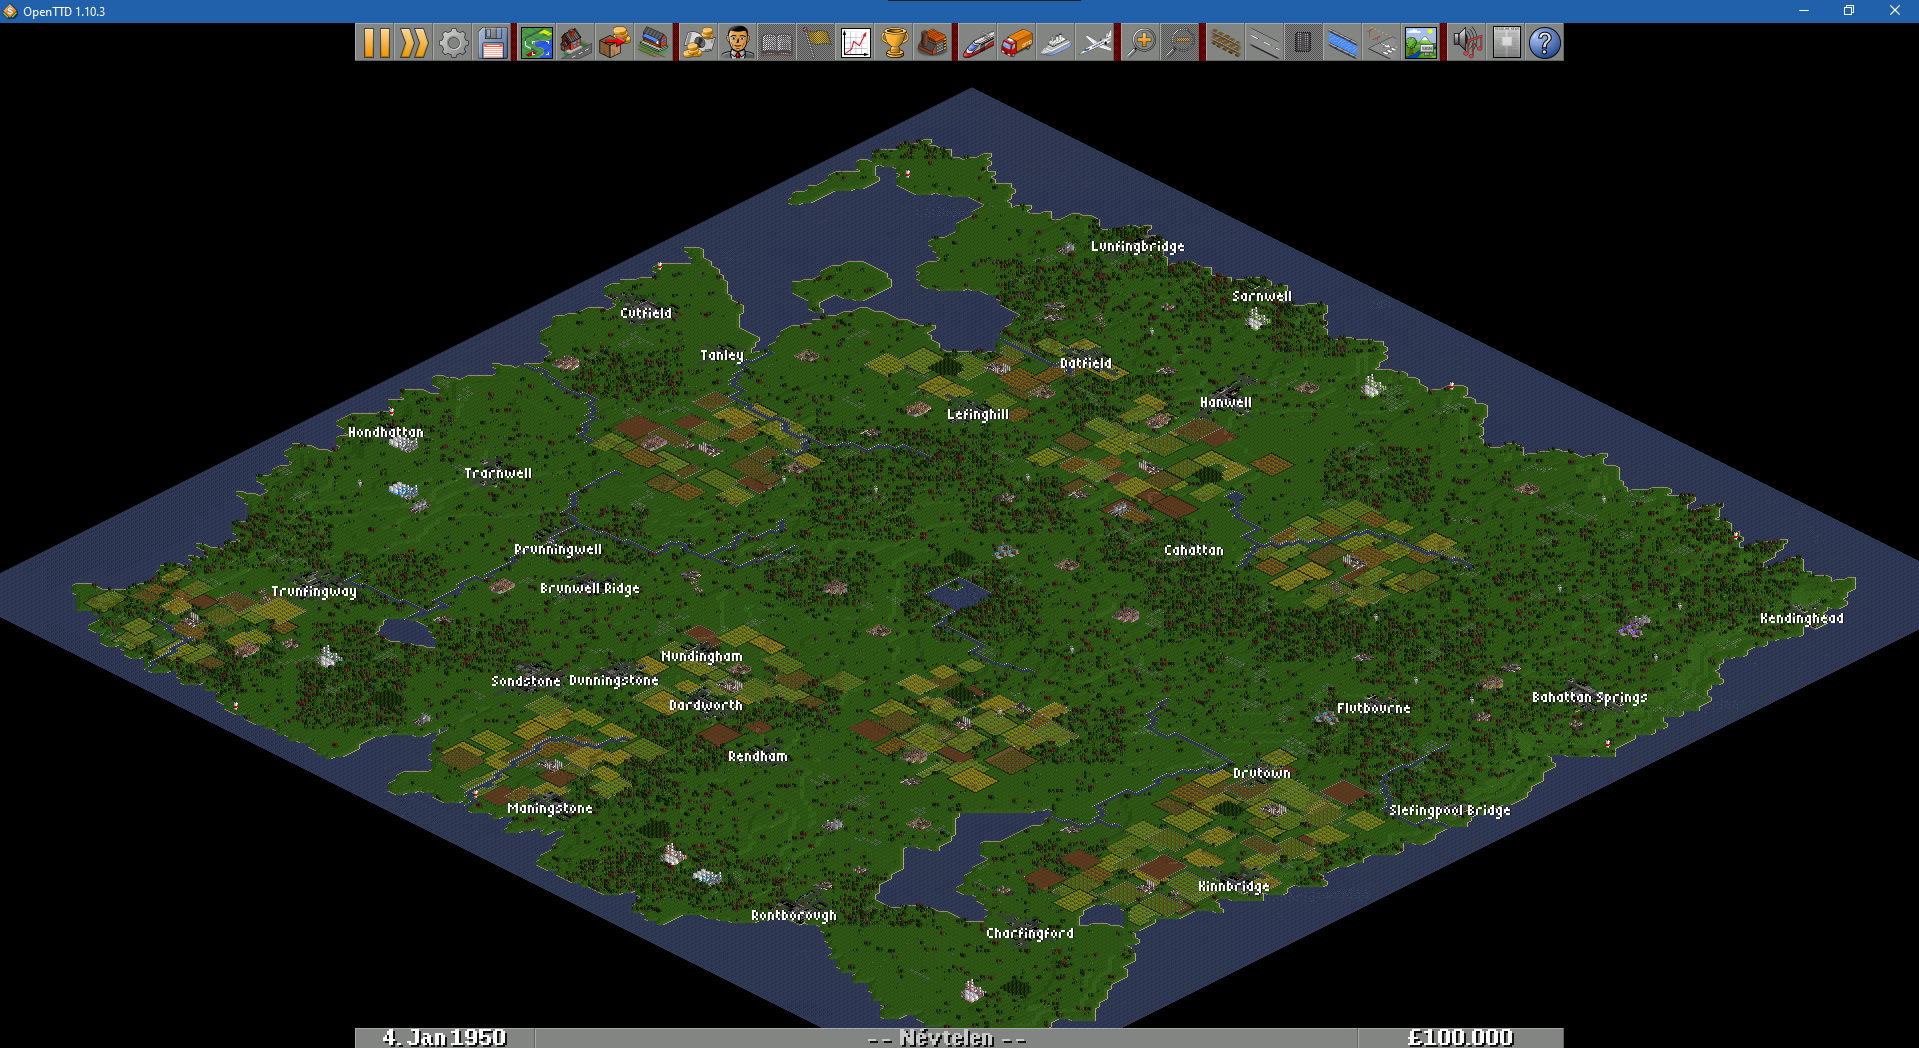
\includegraphics[scale=0.3]{images/palya.png}
	\caption{Egy folyamatban lévő játék felülete, közvetlen a generálás után.}
	\label{fig:palya}
\end{figure}

